
\section{Background}
\label{sec:background}
In this section, we briefly introduce the backlight scaling and WebRTC
for real-time video calls.

\subsection{Backlight scaling}
A visible image on a LCD display is produced by both backlight and the LCD
panel, which stores pixel color imformation. The perceptual luminance
is actually the backlight intensity compensated by the pixels. The
backlight scaling is a technique  exploiting
this characteristic. 
{\bf do we have another figure? captured from playing other videos? If
we do, can replace. But can delay till the last minute.}
Figure~\ref{fig:backlightscaling} sketches the high-level idea. As
shown in the figure, the energy for displaying the image can be
reduced by dimming the backlight. If  nothing else is done, 
 it will lead
to a darker version of this image. This distortion can be compensated
by concurrently increasing the luminance component of each pixel in
this image~\cite{PMLDV03, CHP07, CCS06, CSC02}. And increasing the
pixel brightness does not increase the power consumption of the
display.


\begin{figure}[!htb]
  \begin{center}
    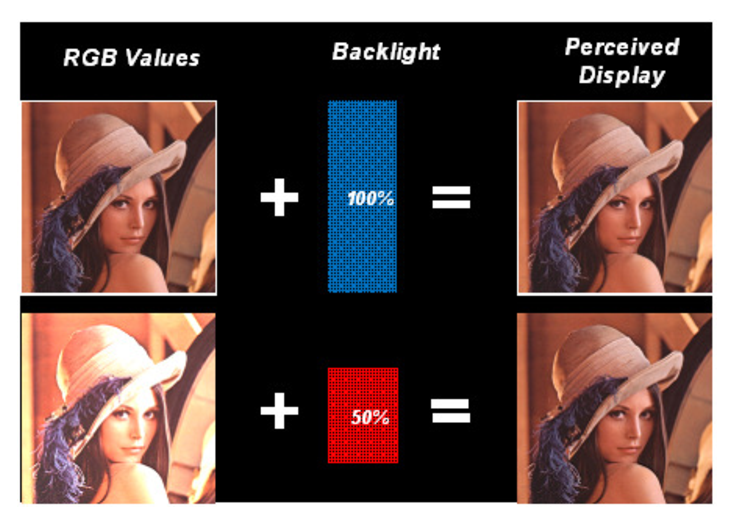
\includegraphics[scale=.75]{./figures/backlightscaling.eps}
    \caption{Backlight Scaling on LCD screen}
    \label{fig:backlightscaling}
  \end{center}
\end{figure}

However, directly applying backlight scaling to video playback faces
several challenges. Both extracting and enhancing the pixels luminance
component frame by frame demand processing a mass of data, and is
computation intensive.  For this reason, deploying these tasks during
the playback on the same CPU~\cite{CHP07, CSC02} is not practical
because of two reasons.  On the one hand, the CPU may not have enough
time to perform these computation intensive tasks without degrading
the video quality (e.g., frames per second or FPS) of the video playback. On
the other hand, the achieved power saving by dimming the backlight can be
offset by the power consumption due to these extra CPU operations. Hsiu et al. and Lin et
al.~\cite{LHH14, HLH11} proposed to skip the pixel compensation stage
and use a critical backlight level for each frame to avoid distorting
the image too badly. Ruggiero et al. suggested to offload the
luminance adjustment tasks to the hardware image processing unit (IPU)
integrated in Freescale’s multimedia application
processor~\cite{RBB08}. It exploits in a smart and efficient way to
implement a hardware assisted image compensation.
%% {\bf is this processor on the same machine or
%%   different machine?} 
Pasricha et al.~\cite{PMLDV03} and Cheng et al.~\cite{CMEDV07}
suggested to compute the backlight scaling data on a proxy server and
substitute the original video with a luminance-adjusted version. In
short, existing schemes (1) only target video-on-demand where the
video frame information is available in advance so that the computing
can be done before the playback, and (2) demand additional
infrastructure support for compensation or do not consider quality
degradation due to backlight dimming. So far, no scheme has been
considered for real-time video calls.

Compared to video-on-demand, real-time video calls are live streaming,
where each frame is produced on the fly and highly
delay-sensitive. Furthermore, video calls often invovle
multiple participants, and thus multiple frames from different sources
needed to be combined in real-time, leaving little computing power for
other tasks, such as pixel luminance compensation.

\subsection{Video Calls and WebRTC}

Video calls/conferecing are gaining increasing popularity.  On mobile
devices, many applications, such as Skype~\cite{skype}, QQ~\cite{qq}, and
Facetime~\cite{facetime}, all support video
calls/conferecing. The communication protocol of these applications is
proprietary to commercial companies, which precludes the communication
between different applications.  The increasing varities of mobile
devices, such as smartphones, tablets and emerging wearable devices,
make the situation even more complicated. To solve this fragmentation
problem in the real-time multimedia communication and also to provide
a cross-platform solution, Web Real-Time Communication
(WebRTC)~\cite{webrtcstandard} is proposed to enable video
communications via web browsers and standardized by the W3C and
IETF. Nowadays, mainstream browsers, e.g., Chrome, Firefox, Opera, all have integrated the WebRTC. The WebRTC
component~\cite{webrtcproject} implemented in the Chrome provides the
Javascript-style APIs. WebRTC can be linked to the native mobile apps
as an external libary.  WebRTC is now widely used by mobile
users. {\bf do you have some data about usage to put here? with
  references.} {\bf revise this later} However, given its video
streaming nature, the power consumption of video communication is
high, which has slowed down its pervasion.



%%% old 
%% \section{background}
%% \label{sec:background}

%% \subsection{Backlight scaling}
%% A visible image on LCD display is produced by both backlight and LCD
%% panel, which stores pixels color imformation. The perceptual luminance
%% is actually the backlight intensity compensated by the pixels. The
%% backlight scaling is a dedicated technique for LCD screen exploiting
%% this characteristics. This technique can be clearly illustrated in the
%% figure~\ref{fig:backlightscaling}. The energy of displaying one
%% picture can only be reduced by dimming the backlight, though it leads
%% to a darker version of this image. This distortion can be compensated
%% by concurrently increasing the luminance component of each pixel in
%% this image~\cite{PMLDV03, CHP07, CCS06, CSC02}. Fortunately, the
%% pixels brightness is uncorrelated to the power consumption of the
%% display.


%% \begin{figure}[!htb]
%%   \begin{center}
%%     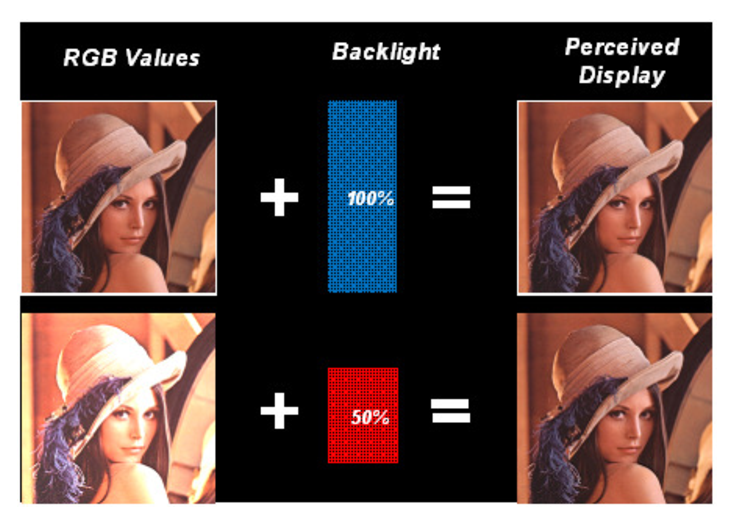
\includegraphics[scale=.75]{./figures/backlightscaling.eps}
%%     \caption{Backlight Scaling on LCD screen}
%%     \label{fig:backlightscaling}
%%   \end{center}
%% \end{figure}

%% Applying this technique in the video playbacks raises several
%% challenges. Both extracting and enhancing the pixels luminance
%% component frame by frame are the operations of processing a mass of
%% data. For this reason, deploying these tasks on the CPU~\cite{CHP07,
%%   CSC02} is not practical. On the one hand, the CPU may don't have
%% enough time to do these computation intensive tasks without degrading
%% the frames per second (FPS) of the video. On the other hand, the
%% achieved power savings by dimming backlight might be offset by these
%% extra operations. Hsiu et al. and Lin et al. ~\cite{LHH14, HLH11} proposed to
%% skip the pixels compensation stage and use a critical backlight level
%% of each frame to avoid distorting the image too badly. Ruggiero et
%% al. offload the luminance adjustment tasks to an independent
%% processor~\cite{RBB08}. Pasricha et al.~\cite{PMLDV03} and Cheng et
%% al.~\cite{CMEDV07} suggested to compute the backlight scaling data on
%% a proxy server and substitute the original video with a
%% luminance-adjusted version.


%% \subsection{WebRTC}

%% The conversational RTC protocols are the company proprietaries,
%% precluding the communication between different services.  The
%% prosperity of mobile devices, including smartphones, tablet
%% and emerging wearable devices, makes the situation more
%% complicated. To solve the fragmentation problem in the real-time
%% multimedia communication and also to provide a cross-platform
%% solution, Web Real-Time Communication (WebRTC)~\cite{webrtcstandard}
%% is proposed and standardized by the W3C and IETF. Nowadays, mainstream
%% browsers, e.g. Chrome, Firefox, Opera and etc., all have integrated
%% the WebRTC inside them. Not only does the WebRTC
%% component~\cite{webrtcproject} implemented in the Chrome provide the
%% Javascript-style APIs, but also it can be linked to the native mobile
%% apps as an external libary. In this paper, we build our prototype
%% based on the AppRTC, which is the Android version app incorperating
%% the WebRTC library.
